\chapter{STEERED}
\label{cha:project}

This chapter focuses on showcasing \textit{STEERED}'s development and implementation.
We start by formalizing the project's goals, showing its purposes and how it could
address real-world problems. Section \ref{sec:project_instrumentation} provides
a detailed description of the instrumentation process, describing how it affects
the produced binary and why it has been designed to work in this way. Section
\ref{sec:project_isr} describes how \textit{STEERED} handles interrupts,
exceptions, and edge controls. Sections \ref{sec:project_ss} and
\ref{sec:project_cfg} show how the Control Flow Graph and the Shadow Stack are
implemented as well as describe how they work. Moreover, Section
\ref{sec:project_pmp}, showcases the configuration for the Physical Memory Protection
used to secure such data structures. Lastly, in Section \ref{sec:project_poc}, a
Proof of Concept is discussed to prove the functioning and security capabilities
of \textit{STEERED}.

\section{Project Formalization}
\label{sec:project_formalization}

\textit{STEERED} aims at providing a secure infrastructure for embedded devices based
on the \textit{RISC-V} ISA. The main goal is to protect the device from control-flow
attacks such as Return-Oriented Programming (ROP) or Jump-Oriented Programming (JOP)
attacks. These cyber-threats attempt to alter the normal execution flow of a
program by jumping or returning to unexpected addresses with the intent of
executing arbitrary code or exfiltrating information. This is even more dangerous
if we consider that small microcontrollers often use only the highest privilege mode
when executing code, as a result, an attacker has a high chance of gaining complete
control over the target device.

To prevent the described attacks, \textit{STEERED} provides a Shadow Stack and a
Control Flow Graph, two data structures used in the security field to enforce
what is called Control Flow Integrity (CFI) which is a security technique that
does not allow the code to perform unexpected control transfer instructions. With
this technique \textit{STEERED} ensure that the software follows the expected
path preventing any unauthorized attempt to alter the execution flow. Moreover,
\textit{STEERED} provides instrumenting capabilities to automatize the implementation
of any code, making the use of the infrastructure easy and fast.

Another goal of \textit{STEERED} is to be as lightweight as possible to meet the
performance requirements of less powerful devices. Thus, great importance is given
to the optimization of both space and time consumption. Moreover, the \textit{RISC-V}
principles have been followed, leaving space for customization of any kind.

To sum up, \textit{STEERED} offers an easy and lightweight infrastructure that makes
it possible to run untrusted code in a secure environment protecting the execution
path of the software and ensures that any control-flow tampering attempt will be
detected by the Control Flow Integrity Enforcer and thus, the device will not be
compromised.

\section{Project Specifics}
\label{sec:project_specifics}

In this section we provide a description of \textit{STEERED} specifics, stating the
utilized tools and files. \textit{STEERED} is published on \textit{GitHub}\cite{repo}
under the \textit{GNU GPL-3.0} license\cite{gpl3} making it freely available to anyone.

The project basic configuration for bare-metal flashing is derived from Sergey Lyubka's
project \textit{mdk}\cite{mdk}, however, we propose a custom flashing solution specifically
developed for \textit{STEERED}. The only requirements to run and flash the code are
\textit{Python v3+} and a toolchain to cross-compile code. During development we
utilized the \textit{riscv-none-elf}\cite{toolchain} toolchain but, with the
proper adjustments, any toolchain can be used. Moreover, since \textit{STEERED}
has been developed and tested on \textit{Espressif's ESP32-C3-DevKitM-1}\cite{esp32c3},
we need to include the \textit{esputil}\footnote{Already available in the GitHub
repository as a submodule\cite{esputil}.} executable to interact with the board \footnote{Note
that if we wish to change the target board, all vendor-specific files must replace
\textit{Espressif}'s files.}.

\begin{wrapfigure}
  [17]{l}{.25\textwidth}
  \centering
  \def\stackalignment{l}\stackunder{ 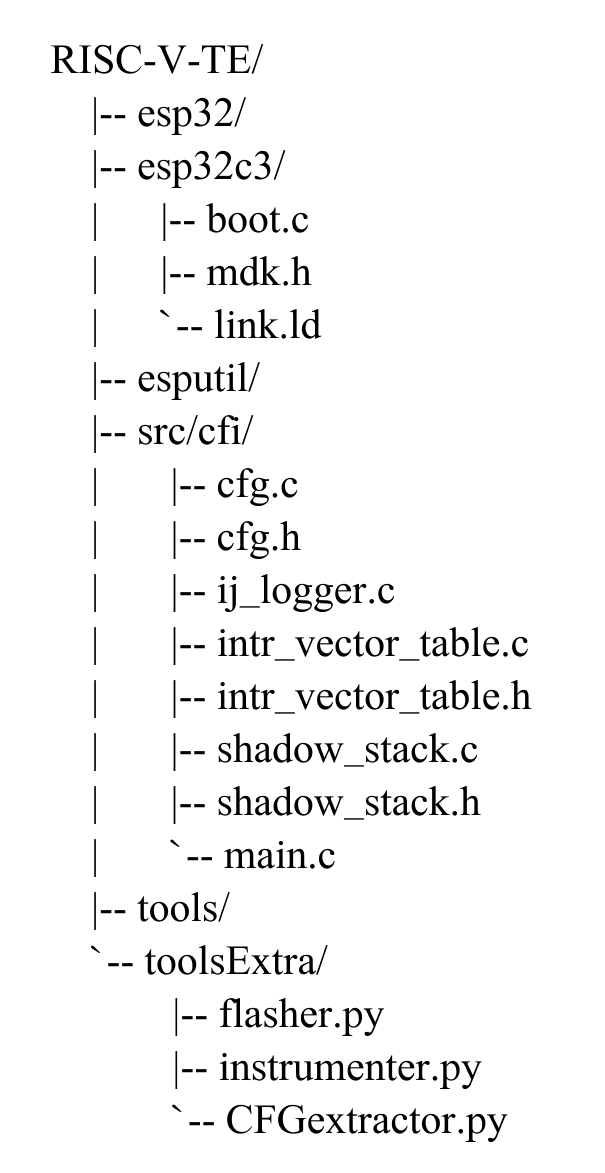
\includegraphics[width=\linewidth]{images/workingtree.png} } %
  {\scriptsize \parbox[t]{\linewidth}{Source: \href{https://github.com/davide-moletta/RISC-V-TE}{GitHub repository}}}
  \caption{\textit{STEERED}'s Working Tree}
  \label{fig:workingtree}
\end{wrapfigure}

Figure \ref{fig:workingtree} depicts \textit{STEERED}'s working tree, where:

\begin{itemize}
  \item \textit{esp32} contains the boot configuration and linker script for
    general \textit{Espressif}'s boards\footnote{Provided by Sergey Lyubka};

  \item \textit{esp32c3} contains the boot configuration and linker script for
    \textit{Espressif's ESP32-C3}\footnote{Provided by Sergey Lyubka but
    severely modified for \textit{STEERED}.};

  \item \textit{esputil} contains \textit{Espressif}'s utils used to manage the board;

  \item \textit{src/cfi/usercode} contains the source files of the untrusted
    code. The files inside this folder will be the target for code instrumentation
    and will be used to produce the secure binary;

  \item \textit{src/cfi} contains the source files for the Shadow Stack, Control
    Flow Graph, interrupt vector table, and machine setup which will be carefully
    described later;

  \item \textit{toolsExtra} contains the \textit{Python} scripts \textit{instrumenter.py},
    \textit{flasher.py}, and \textit{CFGextractor.py} used to instrument, flash,
    and extract the Control Flow Graph respectively (detailed description in Section
    \ref{sec:project_instrumentation}).
\end{itemize}

Inside \textit{src/cfi}, we find the code responsible for managing the machine mode
operations. File \textit{main.c} is responsible for enabling interrupts,
managing privilege modes, and setting up both the Physical Memory Protection (detailed
description in Section \ref{sec:project_pmp}) and the interrupt vector table (detailed
description in Section \ref{sec:project_isr}). File \textit{intr\_vector\_table.c}
is responsible for managing interrupts and exceptions as well as performing both
forward and backward edge controls (detailed description in Section
\ref{sec:project_controls}). Files \textit{cfg.c} and \textit{shadow\_stack.c}
hold the Control Flow Graph and the Shadow Stack configurations respectively (detailed
description in Sections \ref{sec:project_cfg} and \ref{sec:project_ss}). Lastly,
\textit{ij\_logger.c} is used to retrieve indirect jump addresses thanks to a logger.

\subsection{User-Code Importing}
\label{subsec:project_ucodeimport}

During the development of \textit{STEERED} we put great importance on making the
importing of user code easy. Such a process requires only two steps, firstly we need
to copy the needed files inside \textit{src/cfi/usercode}. Once this is done, we
just need to modify the pre-uploaded file \textit{user\_entry.c} located inside the
same folder. The purpose of this file is to make this process faster by
providing a predefined function to modify. By looking at Listing \ref{lst:userentry}
we can see that we only need to call the first function we want to execute of the
imported code to make the project work. \\
\begin{lstlisting}[style=CStyle, caption = \textit{user\_entry.c} File, label={lst:userentry}]
void user_mode_entry_point()
 {
 printf("\n\n--- Start of user code ---\n\n");

 start_u_code(); // Call first user function here

 printf("\n\n--- End of user code ---\n\n");
 }
\end{lstlisting}

\section{Code Instrumentation}
\label{sec:project_instrumentation}

Code instrumentation is the process of modifying software (usually binary or assembly
code) by inserting instructions to perform specific tasks such as a performance
analysis. Instrumentation plays a critical role in this project as it allows to modify
the untrusted code in a simple yet effective way. Moreover, this automatize the process
leading to faster development and reduced number of errors. The whole
instrumentation procedure is depicted in Figure \ref{fig:instrumentation}. \\
\begin{figure}[htbp]
  \centering
  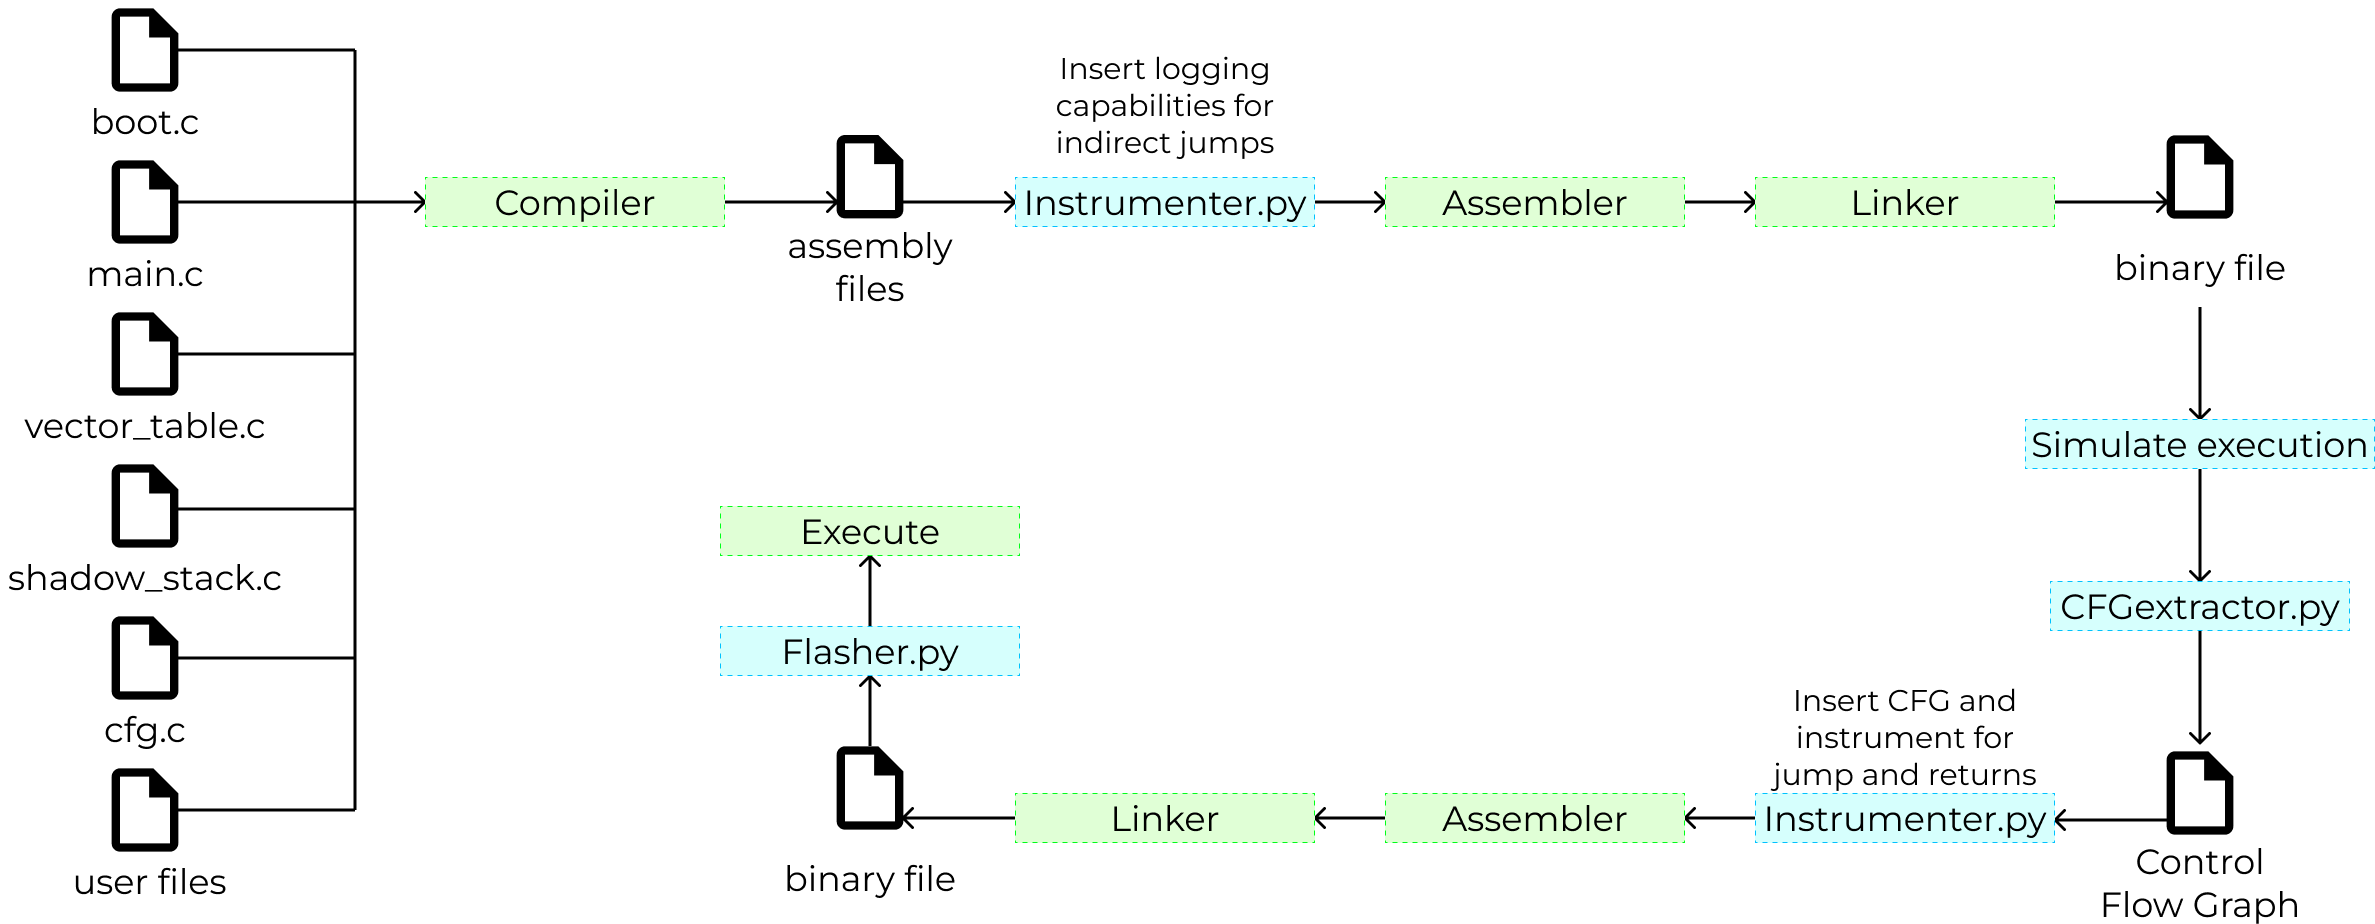
\includegraphics[width=.9\linewidth]{images/instrumentation.png}
  \caption{Flow of the Code Instrumentation Procedure}
  \label{fig:instrumentation}
\end{figure}
\\

In this section, we explain how the \textit{Python} scripts work and how they
can be used to instrument, build, and run the code.

The script \textit{flasher.py} can be run with the command \textit{python3
flasher.py \textbf{command}}, where \textit{\textbf{command}} can be:
\begin{itemize}[noitemsep]
  \item \textit{build}: used to build the source files and produce the binary.
    This command does not provide the security features of \textit{STEERED};

  \item \textit{run}: used to build and run the binary on the target device.
    This command does not provide the security features of \textit{STEERED};

  \item \textit{clear}: used to remove \textit{.bin}, \textit{.elf}, \textit{.s},
    and \textit{.log} files in the directory;

  \item \textit{secure-build}: used to instrument and build the source files and
    produce the secure binary with \textit{STEERED}'s security features;

  \item \textit{secure-run}: used to instrument, build, and run the secure binary
    on the target device with \textit{STEERED}'s security features.
\end{itemize}

As we can see the instrumentation only happens with \textit{secure-build} and \textit{secure-run}
commands. Normal building and running commands have been implemented to make a comparison
between untrusted and trusted code.

The following subsections explain in detail all the steps that occur during the instrumentation
phase.

\subsection{Instrumentation for Logging}
\label{subsec:logging}

Firstly, \textit{flasher.py} takes all the source files and compiles them into
assembly files with the command \textit{riscv-none-elf-gcc -S \{CFLAGS\}\footnote{Utilized
flags are: \textit{-W -Wall -Wextra -Werror -Wundef -Wshadow -pedantic -Wdouble-promotion
-ffixed-a7 -fno-common -Wconversion -march=rv32imc\_zicsr -mabi=ilp32 -O1 -ffunction-sections
-fdata-sections -fno-builtin-printf}.} \{source files\}}. After that, assembly files
of the untrusted user code are passed to \textit{instrumenter.py} for
instrumentation.

In the first step, the code is instrumented with logging capabilities to retrieve
indirect jump destinations. This is done by searching for indirect jump
instructions (\textit{JALR}) with the regex \textit{$\backslash$b(jalr)$\backslash$b$\backslash$s+($\backslash$w+)}
which retrieves any occurrence of \textit{jalr \{register\}}\footnote{Usually
the compiler uses register \textit{a5} for \textit{JALR} instructions.} and
allows us to retrieve the register used to perform the jump.

Once we retrieve the source register for the \textit{JALR} instruction we add the
block of code depicted in Listing \ref{lst:loggingblock} before the jump.

\begin{wrapfigure}
  [27]{r}{0.25\textwidth}
  \setlength{\intextsep}{0pt}
  \begin{minipage}{0.25\textwidth}
    \begin{lstlisting}[style=Assembly, caption = Logging code block, label={lst:loggingblock}]
addi sp,sp,-40
sw a5,4(sp)
sw a4,8(sp)
sw a2,12(sp)
sw a1,16(sp)
sw a0,20(sp)
sw s0,24(sp)
sw s1,28(sp)
sw s2,32(sp)
sw s3,36(sp)
mv a1,{register}
auipc a0,0
addi a0,a0,38
call print_reg
lw a5,4(sp)
lw a4,8(sp)
lw a2,12(sp)
lw a1,16(sp)
lw a0,20(sp)
lw s0,24(sp)
lw s1,28(sp)
lw s2,32(sp)
lw s3,36(sp)
addi sp,sp,40
jalr {register}
 \end{lstlisting}
  \end{minipage}
\end{wrapfigure}

This effectively allows us to save the state of the machine and call the
function \textit{print\_reg} passing the destination address and the program counter
of the \textit{JALR} instruction as arguments. The destination address is simply
retrieved from the source register of the jump instruction and is saved inside register
\textit{a1}. On the other hand, the source address of the jump instruction is
computed by loading the current program counter with \textit{auipc a0, 0} and by
adding $38$\footnote{Note that $38$ is the distance in Bytes from the
instruction that loads the \textit{pc} to the \textit{JALR} instruction.} to it.

When called, the function \textit{print\_reg} prints a string like \textit{Source:
src\_address - Destination: dst\_address} where \textit{src\_address} and
\textit{dst\_address} are the source and destination addresses of the \textit{JALR}
instruction respectively.

\subsection{Control Flow Graph Extraction}
\label{subsec:project_cfgextraction}

After the instrumentation for logging is completed, the assembly files are
assembled and linked to produce the binary with the command \textit{riscv-none-elf-gcc
\{LINKFLAGS\}\footnote{Utilized flags are: \textit{-Tesp32c3/link.ld -nostdlib -nostartfiles
-Wl,--gc-sections}} \{assembly files\} -o output.bin}.

Moreover, if during instrumentation indirect jumps were found in the code, we perform
a ``simulation''\footnote{The simulation consists of running the code on the
target device transparently.} of the execution to retrieve the logging of the
\textit{print\_reg} function.

In any case, the next step involves the extraction of the Control Flow Graph of
the code by calling \textit{CFGextractor.py}. The extraction is performed in two
phases:
\begin{itemize}
  \item Dynamic phase: in the dynamic phase we parse the output retrieved from
    the simulation to create source-destination pairs of addresses. Note that in
    this phase addresses are also adjusted by removing the size of the logging block
    from their value. This is done because, during the simulation we injected the
    logging block before each jump, thus increasing the size of the binary. As a
    result, the retrieved pairs would not match the actual addresses of the
    final binary. So, we compare each address with each block and perform the
    comparison $\textit{address}> \textit{block}$. If the address is higher than
    the current block this means that the block appeared before the instruction so
    we add $1$ to the number of blocks. Once we perform each comparison we can
    compute
    $\textit{final address}= \textit{retrieved value}- (\textit{block size}\footnote
    {Note that the size of each logging block is $56$ Bytes.}* \textit{number of
    blocks})$;

  \item Static phase: in the static phase we simply parse the dump file produced
    with the command \textit{riscv-none-elf-objdump -D output.bin} searching for
    \textit{JAL} instructions. These direct jumps are statically defined in the dump
    file with the following format \textit{\{source address\}: jal \{destination
    address\}} so we just need to extract the needed values. Each time a \textit{JAL}
    instruction is found the pair source-destination is directly added to the
    CFG.
\end{itemize}

Once the Control Flow Graph is extracted, all the pairs are ordered in ascending
order firstly by source and then by destination. This is because, with indirect jump
instructions, we could have more destinations that share the same source. This process
is performed to simplify and optimize the search at run time (detailed
description in Section \ref{sec:project_cfg}). After this step, the execution is
returned to \textit{instrumenter.py} for the final instrumentation phase.

\subsection{Instrumentation for Forward and Backward Edge Controls}
\label{subsec:project_instrcontrols}

In this last instrumentation phase, we need to add code blocks that allow us to
perform forward and backward edge controls. Such blocks must be added before every
direct jump, indirect jump, and return instruction. To do so, we parse the assembly
files, and, search for the target instructions thanks to the Regular Expression (\textit{regex})
functions depicted in Table \ref{tab:regexes}.

\begin{table}
  \centering
  \begin{tabular}{|c|c|}
    \hline
    \textbf{Regex}                                                                      & \textbf{Use}                            \\
    \hhline{==} \textit{$\backslash$b(call)$\backslash$b$\backslash$s+($\backslash$w+)} & Used to find \textit{JAL} instructions  \\
    \hline
    \textit{$\backslash$b(jalr)$\backslash$b$\backslash$s+($\backslash$w+)}             & Used to find \textit{JALR} instructions \\
    \hline
    \textit{$\backslash$b(jr)$\backslash$b$\backslash$s+($\backslash$w+)}               & Used to find \textit{RET} instructions  \\
    \hline
  \end{tabular}
  \caption{\textit{Regex} functions used to find target instructions}
  \label{tab:regexes}
\end{table}

Depending on the instruction we find during parsing we do the following:
\begin{itemize}
  \item \textit{JAL} instructions: if we find a direct jump instruction we need to
    add the code depicted in Listing \ref{lst:dirjumpblock} before the target.
    This code loads the address of the target function in register \textit{a7} and
    then performs an \textit{ECALL} instruction (detailed functioning explained in
    \ref{sec:project_isr}). We use the \textit{load address} (\textit{la}) instruction
    since we need to load the address to which the retrieved label refers to;

  \item \textit{JALR} instructions: if we find an indirect jump instruction we need
    to add the code depicted in Listing \ref{lst:indirjumpblock} before the target.
    This code copies the address stored in the target register into register
    \textit{a7} and then performs an \textit{ECALL} instruction. We use the \textit{move}
    (\textit{mv}) instruction since we need to copy the address from a register to
    another register;

  \item \textit{RET} instructions: if we find a return instruction we need to add
    the code depicted in Listing \ref{lst:retblock} before the target. This code
    copies the return address stored in the return address register into
    register \textit{a7} and then performs an \textit{ECALL} instruction. We use
    the \textit{add immediate} (\textit{addi}) instruction since we need to copy
    the address from one register to another and add $1$. In Section
    \ref{sec:project_isr} we will see why, in this case, we need to add $1$ to
    the return address.
\end{itemize}

\begin{lstlisting}[style=Assembly, caption = Direct jump code block, label={lst:dirjumpblock}]
la a7, {target_function}
ecall
jal {target_function}
\end{lstlisting}

\begin{lstlisting}[style=Assembly, caption = Indirect jump code block, label={lst:indirjumpblock}]
mv a7, {target_register}
ecall
jalr {target_register}
\end{lstlisting}

\begin{lstlisting}[style=Assembly, caption = Return code block, label={lst:retblock}]
addi a7, {return_address_register}, 1
ecall
addi {return_address_register}, a7, -1
ret {return_address_register}
\end{lstlisting}

As soon as the script finishes parsing the dump file it injects the previously
crafted Control Flow Graph into the \textit{cfg.c} file.

After this second instrumentation ends, the modified assembly files are
assembled and linked by \textit{flasher.py} to produce the secure binary file.
Lastly, if we used the \textit{secure-run} command, the binary file is flashed on
the target device for execution.

\section{Machine Setup}
\label{sec:project_setup}

Setting up the machine correctly is fundamental to ensure the correctness of
\textit{STEERED}'s security features. Here, we describe each step needed to configure
the machine in a proper way. \\
\begin{lstlisting}[style=CStyle, caption = Machine setup, label={lst:setup}]
int main(void) {
  asm("la t0, interrupt_vector_table"); // Load vector table address
  asm("ori t0, t0, 1");                 // Set MODE bit to 1
  asm("csrw mtvec, t0");                // Load the address in MTVEC

  asm("csrr t0, mstatus");  // Load MSTATUS in t0
  asm("li t1, 0xFFFFE7FF"); // Load user mode status in t1
  asm("and t0, t0, t1");    // Change MPP bits to user mode
  asm("or t0, t0, 8");      // Change MIE bits to 1
  asm("csrw mstatus, t0");  // Write new MSTATUS

  asm("la t0, user_mode_entry_point"); // Load user mode entry point
  asm("csrw mepc, t0");                // Write new MEPC

  // PMP configuration
  asm("la t0, interrupt_vector_table"); // Load end of first region
  asm("srli t0, t0, 2");                // Shift right
  asm("csrw pmpaddr0, t0");             // Load address in CSR

  asm("la t0, shadow_stack");           // Load end of second region
  asm("srli t0, t0, 2");                // Shift right
  asm("csrw pmpaddr1, t0");             // Load address in CSR

  asm("la t0, .machine_setup");         // Load end of third region
  asm("srli t0, t0, 2");                // Shift right
  asm("csrw pmpaddr2, t0");             // Load address in CSR

  asm("li t0, 0x90000000");             // Load end of fourth region
  asm("srli t0, t0, 2");                // Shift right
  asm("csrw pmpaddr3, t0");             // Load address in CSR

  asm("li t0, 0x0F0B0F0B");             // Load configuration mask
  asm("csrw pmpcfg0, t0");              // Write conf to CSR

  asm("mret"); // Jump to user code in U mode
}
\end{lstlisting}

Referring to Listing \ref{lst:setup} which depicts a simplified version of the \textit{main}
function we see that in lines \textit{2-4} we load the address of the interrupt vector
table in a temporary register. Then, we set \textit{MODE} bit to $1$ to enable
\textit{vectored} mode and we load the proper value inside \textit{mtvec}.

In lines \textit{6-10}, we load the value of \textit{mstatus} inside a temporary
register before modifying it. Firstly, we use a bitmask to modify \textit{machine
previous privilege} bits to U-mode, after that we set \textit{machine interrupt
enable} bits to enable interrupts. Lastly, we load the new \textit{mstatus}.

In lines \textit{12-13}, we load the address of the user mode entry point\footnote{The
first function that needs to be executed in user mode.} inside \textit{mepc}.

After that, the Physical Memory Protection is configured (Detailed description in
Section \ref{sec:project_pmp}) and the instruction \textit{mret} is used to return
execution to the address stored in \textit{mepc} which, in this case, is the
first function of the user code.

Overall, this machine configuration allows us to correctly manage traps thanks to
the interrupt vector table and to configure a secure PMP as well as correctly returning
execution to the user code.

\section{Trap Management}
\label{sec:project_isr}

The purpose of this section is to showcase how the interrupt vector table is
implemented and how interrupts and exceptions are handled inside \textit{STEERED}.
Most importantly we will see how forward and backward edge controls are enforced.

The interrupt vector table is defined inside \textit{intr\_vector\_table.c}. As
already explained its address is loaded in \textit{main.c} and stored inside \textit{mtvec}
(\ref{subsec:riscv_mtvec}) with \textit{MODE} set to vectored. This means that
every asynchronous interrupt will set the program counter to the base address of
the interrupt vector table plus $4$ times the cause of the interrupt. Any other interrupt
and exception is trapped inside the function \textit{synchronous\_exception\_handler}
which redirects to the correct function depending on the trap cause. Listing \ref{lst:intrtable}
depicts the actual implementation of the interrupt vector table.

Most of the exceptions and interrupts are not currently handled and, when
invoked, they just log a message describing which trap was taken before resuming
the execution. This design choice has been made for two reasons. The first is that
such implementation would be out of scope since we aim at providing the bare minimum
implementation for enforcing Control Flow Integrity. The second instead is that
we do not need those handlers and we leave space for implementation-specific
requirements. For example, if a future implementation makes use of external
interrupts, the developer would just need to insert the desired handling in the correct
function inside the \textit{intr\_vector\_table.c} file. As explained, this
implementation provides the required security features while leaving space for
customization.

Since \textit{ECALL}s are defined as exceptions in \textit{RISC-V}, the
interrupt vector table is responsible for managing them. For this reason, the
only implemented function inside \textit{intr\_vector\_table.c} is the handler for
U-mode \textit{ECALL}s. This implementation is tailored for managing forward and
backward edge controls. However, since \textit{ECALL}s can be used for different
purposes the handler is designed to be expandable. Table \ref{tab:ecalls} depicts
the current allowed ecalls.
\begin{table}
  \centering
  \begin{tabular}{|c|c|c|}
    \hline
    \textbf{Code}                & \textbf{Use}     & \textbf{Description}                  \\
    \hhline{===} $1$             & Reserved         & Used to terminate execution           \\
    \hline
    \textit{destination address} & Forward control  & Used to check the destination address \\
    \hline
    $\textit{return address}+ 1$ & Backward control & Used to check the return address      \\
    \hline
  \end{tabular}
  \caption{Encoding of currently allowed \textit{ECALL} values}
  \label{tab:ecalls}
\end{table}
\\
\begin{lstlisting}[style=CStyle, caption = Interrput Vector Table, label={lst:intrtable}]
void interrupt_vector_table(void) {
 asm volatile("j synchronous_exception_handler");
 asm volatile("j isr_supervisor_software");
 asm volatile("j isr_reserved");
 asm volatile("j isr_machine_software");
 asm volatile("j isr_user_timer");
 asm volatile("j isr_supervisor_timer");
 asm volatile("j isr_reserved");
 asm volatile("j isr_machine_timer");
 asm volatile("j isr_user_external");
 asm volatile("j isr_supervisor_external");
 asm volatile("j isr_reserved");
 asm volatile("j isr_machine_external");
 asm volatile("j isr_reserved");
}
\end{lstlisting}

Currently, the U-mode \textit{ECALL} handler is implemented as depicted in Listing
\ref{lst:ecallhandler}. As it is possible to see we encoded the \textit{ECALL} code
and the address required for edge controls into a single value. This design has
been used to minimize the use of registers. Another solution would have been to use
a register, say \textit{a7}, to hold the \textit{ECALL} code, and another
register, say \textit{a6}, to hold the address to check. However, since legal addresses
must be even we can encode in one register both the value of the \textit{ECALL}
code and the address using the otherwise unused least significant bit (Figure \ref{fig:ecall}
shows the encoding of register \textit{a7}). When the interrupt vector table
needs to check which code is used we can just see if the value in \textit{a7}\footnote{In
Listing \ref{lst:ecallhandler} register \textit{a7} is represented by the parameter
\textit{ecode}.} is even or odd and, depending on the result, we can decide
which operation to perform\footnote{Even values will lead to a forward edge
check while odd values will lead to a backward edge check.}. When we need to
check for a return address we first subtract $1$ from it to obtain the original
value of the address and then we perform the control. \\
\begin{figure}[htbp]
  \centering
  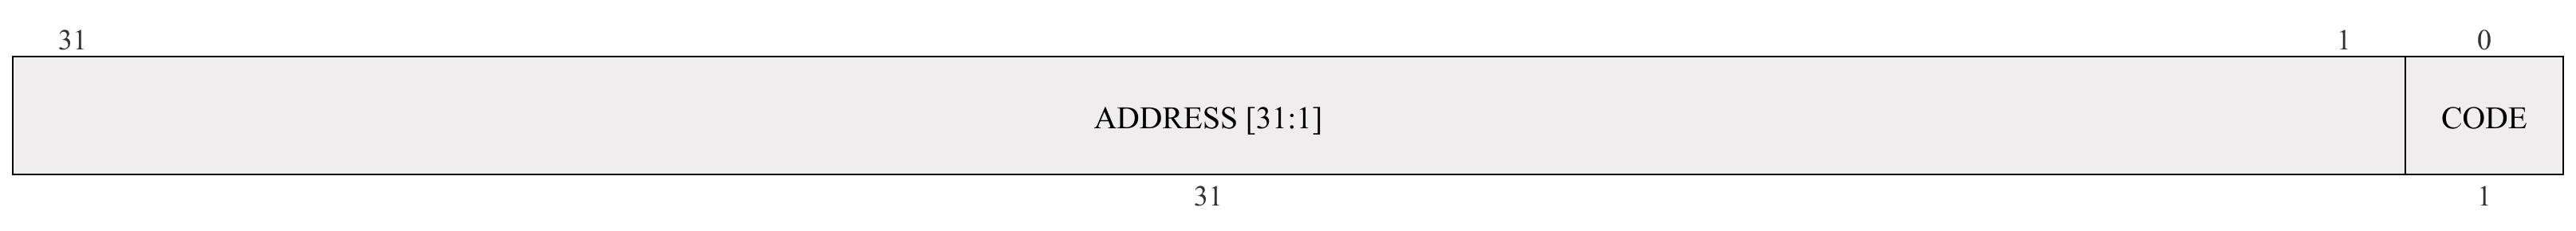
\includegraphics[width=.9\linewidth]{images/ecall_code.png}
  \caption{Encoding of register a7 during \textit{ECALL}}
  \label{fig:ecall}
\end{figure}
\\

Note that the use of register \textit{a7} to hold \textit{ECALL} codes is purely
a design choice and, to ensure that such register is not tampered with by the compiler
it has been ``disabled'', meaning that the compiler will never use such register.
This choice allows us to be sure that only the interrupt vector table and the code
blocks that we inject modify the value of \textit{a7}. Another solution would have
been to let the compiler use register \textit{a7} and, during the instrumentation
phase, check for its usage. When used we could inject more instructions to store
the previous value in the stack and then retrieve it after the edge control.
However, since we wanted to inject as few instructions as possible to avoid impacting
too much on the performance the first solution has been implemented.

If one wishes to add a new custom \textit{ECALL} code for other purposes he just
needs to put a control before the handler checks if the \textit{ecode} is even or
not. Say that we want to add code $2$ to perform a specific operation. To do so,
we just need to add a check like \textit{else if(ecode == 2) \{perform operation\}}
after the first check, if the check fails the code will eventually check if the
code is even or not and perform the corresponding edge control.

It is easy to see how this implementation effectively allows to manage any trap
while addressing the problem and leaving space for possible future customization
of the interrupt vector table. \\ \begin{lstlisting}[style=CStyle, caption = U-mode \textit{ECALL} handler, label={lst:ecallhandler}]
void esr_handler_U_mode_ecall(u_int ecode, u_int mepc) {
  if (ecode == 1) {
    code_termination();
  } else if ((ecode % 2) == 0) {  // Forward edge control
    u_int source = mepc + 4;      // Source address

    // Check if address is inside the CFG
    if (check(source, ecode)) {
      if (push(source + 2) != 1){ // Try push into Shadow Stack
        code_termination();       // Push failed
      }
    } else {
      code_termination();         // CFG check failed
    }
  } else if ((ecode % 2) != 0) {  // Backward edge control
    u_int pop_addr = pop();       // Popped address

    // Compare popped address with return address
    if (pop_addr == 0 || pop_addr != ecode - 1) {
      code_termination();         // Check failed
    }
  } else {
    // Undefined ecode, log and return
  }
}
\end{lstlisting}

Forward edge controls are performed thanks to the Control Flow Graph and are
further explained in section \ref{sec:project_cfg} while backward edge controls
are performed thanks to the Shadow Stack and are further explained in section
\ref{sec:project_ss}.

\section{Shadow Stack}
\label{sec:project_ss}

In \textit{STEERED}, the Shadow Stack holds the values of return addresses and it
is used to check the correctness of each \textit{RET} instruction. File \textit{shadow\_stack.c}
holds the configuration for the Shadow Stack. The development of the said data structure
took inspiration from the formally verified idea proposed by Matthieu Baty,
Guillaume Hiet, and Pierre Wilke in their article \textit{Work in progress: A formally
verified shadow stack for RISC-V} \cite{shadowstack}. In their article, they
demonstrate a methodology for formally specifying and verifying the correctness
of a Shadow Stack implemented in \textit{RISC-V}. Their approach involves the
use of formal methods and the hardware description language \textit{Kôika}\cite{koika}
to prove the integrity of the Shadow Stack against return address manipulation. The
authors also discuss the isolation of the Shadow Stack from regular memory access,
ensuring robust protection against tampering, and provide a verified framework that
halts execution if a violation is detected, such as a stack overflow or an
invalid return address. This rigorous approach highlights the importance of formal
verification in designing secure hardware systems, which served as a
foundational inspiration for our implementation.

The Shadow Stack is implemented as a standard Last-In-First-Out (\textit{LIFO}) stack.
This design choice has been made to provide a data structure with fast lookups\footnote{Lookups
in the Shadow Stack are performed in $\mathcal{O}(1)$.} while maintaining the ability
to use fewer space when return addresses are not needed. This implementation is
possible only because the last jump instruction that is performed in a code will
always be the first to return. Otherwise, it would be necessary to store each
return address and its relative jump instruction to know which address we need
to check each time. This allowed us to build an effective and fast data structure
that consumes a variable amount of memory, rarely affecting the execution
performance.

The Shadow Stack is statically defined as a \textit{C} struct that contains an array
which can hold up to $63$ addresses and a pointer to the top index of the stack (Listing
\ref{lst:ss} shows the described struct). Moreover, the file \textit{shadow\_stack.c}
allows two operations, \textit{push} and \textit{pop} where:
\begin{itemize}
  \item \textit{Push} is used during a forward edge control. If such control succeeds
    then, the return address related to the jump instruction is pushed into the
    Shadow Stack and stored\footnote{Addresses are stored in the Shadow Stack as
    \textit{unsigned integers}.} for later use. In this case, we just use the stack
    pointer to determine if the Shadow Stack can accommodate more addresses. If
    the Shadow Stack is full, and no other addresses can be stored, we terminate
    execution immediately as we can't provide the necessary data for the next
    backward edge control. Otherwise, the address is added to the top of the
    stack and the execution continues normally;

  \item \textit{Pop} is used when we need to perform a backward edge control. When
    this happens, an address is removed from the top of the Shadow Stack. Afterwards,
    we match the removed address with the user-provided return address to decide
    whether the return instruction is considered legal or not\footnote{Note that
    when we use \textit{pop} we actually remove the element from the stack since
    we won't need it in the future and, by doing this, we can free some space in
    the data structure.}. Note that before removing the address we check if the
    Shadow Stack is empty and, if that is the case, we terminate execution
    immediately since the code is trying to perform an unexpected return
    instruction.
\end{itemize}

The Shadow Stack provides no other functions for two main reasons. Firstly, with
\textit{push} and \textit{pop} we have all we need to effectively make the controls
we need and. Secondly, because by adding extra functions not only we increase the
binary size, but we could also accidentally insert weak code inside the binary
that may lead to unexpected behavior.

Note that the size of the Shadow Stack can be adjusted to fit every need by
simply modifying the value of \textit{MAX\_SIZE} inside \textit{shadow\_stack.c}.
For example, if we know that our code will never nest for more than $5$ times we
can reduce the size of the Shadow Stack to $6$ since we are sure that we will
never have more than $5$ jump instructions consecutively. \\ \begin{lstlisting}[style=CStyle, caption = Shadow Stack definition inside \textit{shadow\_stack.c}, label={lst:ss}]
#define MAX_SIZE 63

typedef struct {
  u_int addresses[MAX_SIZE]; // Array used to store return addresses
  int top;                   // Pointer to the top of the stack
} SStack;
\end{lstlisting}

\section{Control Flow Graph (CFG)}
\label{sec:project_cfg}

In \textit{STEERED}, the Control Flow Graph holds the pair source-destination for
each direct and indirect jump of the code and it is used to check the correctness
of each \textit{JAL} and \textit{JALR} instruction. As already said the CFG of
the binary is extracted during the instrumentation phase and injected into the
file \textit{cfg.c} which holds the configuration for the Control Flow Graph (Listing
\ref{lst:cfgdefinition} depicts the current representation of the Control Flow
Graph). \\
\begin{lstlisting}[style=CStyle, caption= Definition of the Control Flow Graph inside \textit{cfg.c}, label={lst:cfgdefinition}]
u_int cfg[][2] = {{src, dst}, ...}; // Source-destination pairs
size_t cfg_size = 1;                // Size of the CFG
\end{lstlisting}

It is worth noting that the CFG is related only to control transfer instructions
of the untrusted code. This is because we need to enforce Control Flow Integrity
only on U-mode code, thus not saving the CFG of all the binary helps in reducing
memory usage. Moreover, the Control Flow Graph does not hold the values of return
addresses, this is because return instructions are checked thanks to the Shadow
Stack, thus we do not need to save those values in the CFG. These design choices
allowed us to create a tailored structure that is both fast and efficient in
space usage.

Inside \textit{cfg.c}, we can see the structure of the Control Flow Graph which
is composed of a two dimensional array where, each index represents an edge.
Such edge is stored in a small array that contains the source address in the
first position and the destination address in the second position. So, the CFG
holds a pair \textit{source-destination} at each position, moreover, as explained
in section \ref{sec:project_instrumentation}, the pairs are ordered in non-decreasing
order during the instrumentation phase. The \textit{cfg.c} file provides only
the \textit{check} function which asks for a pair of addresses as input and determines
whether such a pair is part of the Control Flow Graph or not. \textit{check} is implemented
using a binary search algorithm with a custom comparison function (Listing
\ref{lst:binsearch} depicts a representation of the compare function). We needed
to create a custom compare function because we need to perform the binary search
with two values (source and destination addresses), thus a normal comparison would
not work in this scenario. With this function we firstly search the source
address and then, if we find a match, we search for the destination address. Note
that this approach is possible only because the list was previously ordered,
otherwise the binary search would not work correctly and we would need to
perform a linear search which would result in a time complexity of
$\mathcal{O}(n)$. Lastly, if the binary search finds a match, the \textit{check}
function returns a positive value and the jump instruction is considered legal. \\
\begin{lstlisting}[style=CStyle, caption= Comparison for binary search, label={lst:binsearch}]
  int compare(const int* A, const int* B) {
    for (int i = 0; i < 2; ++i) {
      if (A[i] < B[i]) return -1;
      if (A[i] > B[i]) return 1;
    }
    return 0;
  }
\end{lstlisting}

Since the CFG will not change during execution we can define it statically and
provide no functions to add or remove elements. Again, the reason behind this
choice is to reduce memory usage and to avoid the implementation of unused
functions.

This implementation of the Control Flow Graph effectively reduces space
consumption to the bare minimum while providing fast lookups with a time
complexity of $\mathcal{O}(\log{n})$\footnote{Note that since the Control Flow
Graph will never reach enormous sizes like $10^{5}$ we can approximate the time
complexity of $\mathcal{O}(\log{n})$ to $\mathcal{O}(1)$.}. Another solution
could be to use a hash table to store the address pairs. In this case, we would
reduce the time required to access the CFG to $\mathcal{O}(1)$ for any size of
the CFG since accesses to hash tables are instantaneous. However, this works
only with big enough hash tables, otherwise, we could face many collisions, and the
time required to find the correct entry would increase. This means that we would
need to allocate a lot of space to store few addresses leading to a waste of
memory usage since most of the entries would be empty. Still, this alternative
solution could be perfect for situations in which we care more about time than
space.

\section{Memory Layout}
\label{sec:layout}

The purpose of this section is to discuss the memory layout of the binary (Listing
\ref{lst:linker} depicts a simplified version of the linker script used to
compile the code). \\
\begin{lstlisting}[style=CStyle, caption= Simplified linker script, label={lst:linker}]
  MEMORY {
    iache (rwx): ORIGIN = 0x4037c000, LENGTH = 16k
    iram  (rwx): ORIGIN = 0x40380400, LENGTH = 32k
    dram  (rw): ORIGIN = 0x3fc80000 + LENGTH(iram), LENGTH = 128k
  }

  ENTRY(_start)

  SECTIONS {
    .interrupt_vector_table: {*(.interrupt_vector_table)} > iram

    .intr_service_routines: {*(.intr_service_routines)} > iram

    .shadow_stack: {*(.shadow_stack)} > iram

    .cfg: {*(.cfg)} > iram

    .machine_setup: {*(.machine_setup)} > iram

    .text: {*(.text) *(.text*)} > iram

    .ij_logger: {*(.ij_logger)} > iram

    .data: {*(.data*) *(.sdata*) *(.srodata*) *(.rodata*)} > dram
  }
\end{lstlisting}

Each part of the codebase has been assigned to separate sections as follows:
\begin{itemize}
  \item Section \textit{.interrupt\_vector\_table} holds the interrupt vector
    table function described in \ref{lst:intrtable};

  \item Section \textit{.intr\_service\_routines} holds the exception and
    interrupt handlers as well as the functions to interact with the Shadow
    Stack and the Control Flow Graph;

  \item Section \textit{.shadow\_stack} holds the data structure related with
    the Shadow Stack;

  \item Section \textit{.cfg} holds the data structure related with the Control
    Flow Graph;

  \item Section \textit{.machine\_setup} holds the boot setup functions and the
    \textit{main} function;

  \item Section \textit{.text} holds the untrusted code;

  \item Section \textit{.ij\_logger} holds the function \textit{logger} used to log
    indirect jump addresses during the simulation.
\end{itemize}

This configuration has been implemented to increase granularity between all the parts
of the code. Moreover, as we will see in section \ref{sec:project_pmp}, such
configuration allows for an easier and more effective definition of the Physical
Memory Protection.

As we can see, execution starts at function \textit{\_start} which is located
inside the file \textit{boot.c}. Such function initializes the device and
transfers execution to the \textit{main.c} file which sets up all the M-mode configurations
before starting the user code.

\section{Physical Memory Protection (PMP)}
\label{sec:project_pmp}

In this project, the role of Physical Memory Protection is to protect the Shadow
Stack and the Control Flow Graph from unauthorized access and modification (the
PMP definition is depicted in Listing \ref{lst:setup}). To ensure that both
these data structures are secured four memory regions have been created (each region's
configuration can be seen in Table \ref{tab:pmpregions}).

The four regions are designed to cover different memory sections and provide
different privileges:
\begin{itemize}
  \item Region $1$: the first region covers all the memory space between
    $0x00000000$ and the end of the \textit{.data} region. This part of memory
    has been granted with read and write privileges, since this region contains only
    static data there is no need to allow execution. To configure this region we
    used the instruction \textit{la t0, interrupt\_vector\_table} to load the address
    of the \textit{.interrupt\_vector\_table} section which follows the \textit{.data}
    section. Afterwards, we used \textit{srli t0, t0, 2} to make a right shift
    as it is required by \textit{RISC-V}. Lastly, we load the address in \textit{pmpaddr0}
    with the instruction \textit{csrw pmpaddr0, t0}. Note that we load the
    address of the section that follows \textit{.data} because with a TOR configuration
    the upper address determines the end of the PMP section;

  \item Region $2$: the second region covers the interrupt vector table and all
    the exceptions and interrupts handlers as well as CFG and Shadow Stack
    functions, since this region is accessed only in Machine mode and we need to
    execute instructions we need to provide read, write, and instruction execution
    privileges. To configure this region we used the instruction \textit{la t0, shadow\_stack}
    to load the address of the \textit{.shadow\_stack} section which follows the
    \textit{.interrupt\_service\_routine} section. Afterwards, we used \textit{srli
    t0, t0, 2} to make a right shift as it is required by \textit{RISC-V}.
    Lastly, we load the address in \textit{pmpaddr1} with the instruction
    \textit{csrw pmpaddr1, t0};

  \item Region $3$: the third region is the one that covers both the Shadow
    Stack and the Control Flow Graph. For this reason, we need to restrict
    privileges to read and write only. We can't set this region as read-only since
    we need to modify the Shadow Stack during execution. Note that the \textit{.shadow\_stack}
    and \textit{.cfg} sections only cover the data structures related to the
    Shadow Stack and Control Flow Graph respectively. \textit{Push}, \textit{pop},
    and \textit{check} are categorized as ``handlers'', thus those functions are
    inserted in the \textit{.intr\_service\_routine} section. This is because we
    need instruction execution privileges for said functions to work. To
    configure this region we used the instruction \textit{la t0, .machine\_setup}
    to load the address of the \textit{..machine\_setup} section which follows
    the \textit{.cfg} section. Afterwards, we used \textit{srli t0, t0, 2} to
    make a right shift as it is required by \textit{RISC-V}. Lastly, we load the
    address in \textit{pmpaddr2} with the instruction \textit{csrw pmpaddr2, t0};

  \item Region $4$: the fourth and last region covers all the addresses from the
    start of the main function up to the end of the memory. This region also includes
    user code and, since we need to execute the code, we need to configure this region
    with read, write, and instruction execution privileges. To configure this
    region we used the instruction \textit{li t0, 0x900000000} to load the value
    $0x90000000$ which represent the end of the memory. Afterwards, we used \textit{srli
    t0, t0, 2} to make a right shift as it is required by \textit{RISC-V}.
    Lastly, we load the address in \textit{pmpaddr3} with the instruction
    \textit{csrw pmpaddr3, t0}. Note that there is no need to separate user code
    from the machine setup as they need the same privileges during execution\footnote{Referring
    to PMP privileges, not actual execution privileges}.
\end{itemize}

Lastly, we use the instructions \textit{li t0, 0x0F0B0F0B} and \textit{csrw
pmpcfg0, t0} to load the configuration of the four memory regions. The value
$0x0 B0F0B0F$ represent the privileges and type of each memory region. Referring
to section \ref{sec:riscv_pmp}, we have:
\begin{itemize}
  \item $0F$ or $00001111$: used to configure the fourth region as a TOR section
    with read, write, and instruction execution privileges;

  \item $0B$ or $00001011$: used to configure the third region as a TOR section
    with read and write privileges;

  \item $0F$ or $00001111$: used to configure the second region as a TOR section
    with read, write, and instruction execution privileges;

  \item $0B$ or $00001011$: used to configure the first region as a TOR section
    with read and write privileges.
\end{itemize}

Note that the value of the configuration is read backwards because \textit{RISC-V}
interprets this value as little endian.

This Physical Memory Protection configuration effectively helps to prevent unauthorized
modifications to critical components such as the Shadow Stack and the Control Flow
Graph. Thanks to this, we are sure that whatever value we read from these data structures
will be safe and trustable. Note that any access made from U-mode to the third
memory region will result in either an \textit{Instruction Access Fault} or an \textit{Illegal
Instruction} exception.

\begin{table}
  \centering
  \begin{tabular}{|c|c|c|c|c|}
    \hline
    \textbf{Region}    & \textbf{Region Start}                             & \textbf{Region End}              & \textbf{Type} & \textbf{Privileges} \\
    \hhline{=====} $1$ & $0x00000000$                                      & \textit{.data} ($0x40380400$)    & TOR           & R-W                 \\
    \hline
    $2$                & \textit{.interrupt\_vector\_table} ($0x40380400$) & \textit{.intr\_service\_routine} & TOR           & R-W-X               \\
    \hline
    $3$                & \textit{.shadow\_stack}                           & \textit{.cfg}                    & TOR           & R-W                 \\
    \hline
    $4$                & \textit{.machine\_setup}                          & $0x90000000$                     & TOR           & R-W-X               \\
    \hline
  \end{tabular}
  \caption{PMP memory regions}
  \label{tab:pmpregions}
\end{table}

\section{Forward and Backward Edge Controls}
\label{sec:project_controls}

The most critical job of \textit{STEERED} is validating jump and return instructions
with the U-mode \textit{ECALL} handler located inside the \textit{intr\_vector\_table.c}
file. Given the delicacy of Control Flow Integrity and its importance for this
project, great attention has been given to the correct implementation of forward
and backward edge controls.

As already explained in sections \ref{sec:project_ss} and \ref{sec:project_cfg},
forward and backward edge controls are performed thanks to the Control Flow
Graph and Shadow Stack respectively. However, in this section, each control will
be carefully explained to show how it works and why it provides a certain degree
of security to the project.

\subsection{Forward Edge Controls}
\label{subsec:forward}

A forward edge control is performed to check whether a direct or indirect jump
instruction is trying to transfer control from a legal address to a legal
address. In our case, legality is determined by the fact that the jump stays in
the address range related to user code and that the pair source-destination is
contained in the Control Flow Graph.

To perform a forward edge control we need three things. Firstly, we need both
the source and destination addresses of the jump instruction we want to check. Lastly,
we need a trusted oracle that tells us if the pair source-destination is legal. As
already explained the destination address is retrieved from \textit{a7} which is
passed as the \textit{ECALL} code. The source address instead can be retrieved
from \textit{mepc} \ref{subsec:mepc}. As we have seen, when a trap is taken \textit{mepc}
is written with the address of the instruction that was interrupted. Since in \textit{RISC-V}
an \textit{ECALL} generates a trap, we can just add $4$ to the address stored in
\textit{mepc} to retrieve the source address of the jump instruction\footnote{We
add $4$ since it is the size of an \textit{ECALL} instruction in \textit{RISC-V}.}.
Now that we have the needed pair of addresses to check we can use the Control Flow
Graph as the oracle. As already explained, the CFG is computed before compilation
and is securely stored in a safe memory region thanks to Physical Memory Protection.
This means that any attempt of unauthorized modification is instantly blocked, thus
so we can trust the data provided by the CFG and use it as an oracle.

When we need to perform a forward edge control, we just send the source and
destination addresses to the \textit{check} function of the CFG. Such function
performs a binary search inside the Control Flow Graph to see whether that
specific pair is part of the original CFG or not. If the search succeeds the function
returns a positive value and the jump is considered legal while, if the search
does not succeed the instruction is aborted and the execution terminates to
prevent any possible damage.

Whenever a forward edge control succeeds we know that the related jump
instruction will eventually return so we need to store its return address inside
the Shadow Stack. To do so, we need to retrieve the return address but, since a jump
will always return to its next instruction, we can just compute
$\textit{source address}+ 2$ to retrieve it\footnote{We add $2$ since it is the
size of compressed \textit{JAL} and \textit{JALR} instructions in \textit{RISC-V}.}.
After that, the return address is pushed into the Shadow Stack and the execution
is resumed with the interrupted jump instruction. Note that the execution is
resumed if and only if the Shadow Stack has room for the pushed address, otherwise
we abort the operation and terminate execution.

\subsection{Backward Edge Controls}
\label{subsec:backward}

A backward edge control is performed to check whether a return instruction is
trying to transfer control from a legal address to a legal address. In our case,
legality is determined by the fact that the return stays in the address range
related to user code and that the return address is the last address that was
pushed into the Shadow Stack.

To perform a backward edge control we need two things. Firstly, we need the
address to which the return instruction is trying to transfer control. Secondly,
we need a trusted oracle that tells us if such an address is legal. As we have seen,
the destination address is retrieved from \textit{a7} which is passed as the \textit{ECALL}
code. However, we must remove $1$ from the address retrieved from \textit{a7} since
in the least significant bit we store the \textit{ECALL} code. Similarly to the Control
Flow Graph, the Shadow Stack is secured in a protected memory space and is
unaffected by unauthorized modification attempts. Even in this case we can trust
the Shadow Stack and use it as an oracle.

When we need to perform a backward edge control, we just need to \textit{pop} an
address from the Shadow Stack and match the destination address of the return instruction
with the popped one. If the addresses are different the execution is terminated
as the code is trying to return to an unauthorized address while, if the addresses
are equal, we can consider the return instruction legal and resume execution
with the interrupted return instruction.

Whenever a backward edge control succeeds we must do nothing since the value has
already been removed from the Shadow Stack and no other modifications are needed.

We must note that backward edge controls could be implemented in another way. If
we need to control a return address and there is a mismatch we could force the user
code to return to the address stored in the Shadow Stack which we know is safe.
While this solution enforces Control Flow Integrity securely we can't be sure
that the stack\footnote{Referring to the normal stack used to store registers} has
not been compromised and thus, terminating execution is a much safer choice.

\section{Proof of Concept (PoC)}
\label{sec:project_poc}

In this section, we provide a Proof of Concept to showcase how \textit{STEERED} effectively
provides security capabilities to a non-trusted and insecure code. Figure
\ref{fig:functioning} depicts an abstraction of the project's flow where green
and red boxes depict trusted and untrusted components respectively. Moreover,
green arrows are used to represent a successful edge control while red arrows
represent an unsuccessful one. \\
\begin{figure}[htbp]
  \centering
  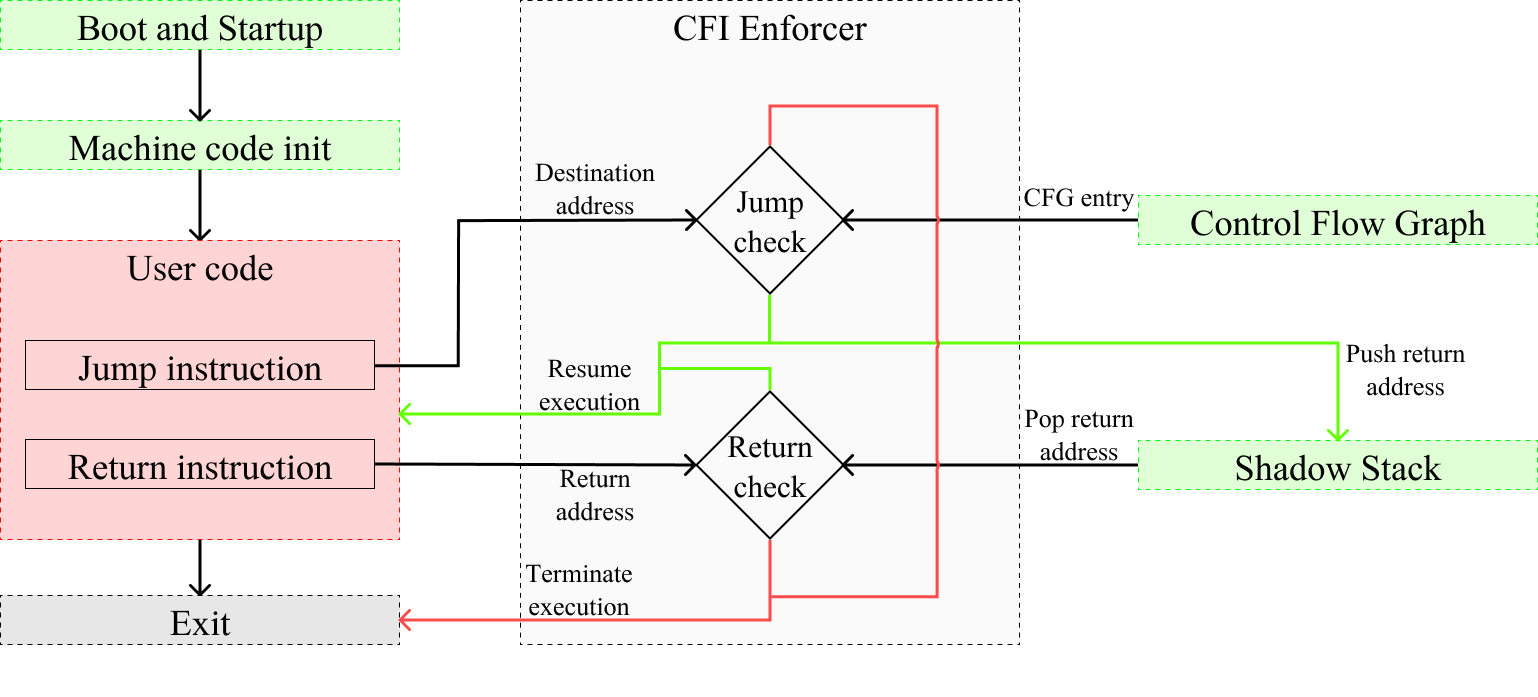
\includegraphics[width=.9\linewidth]{images/functioning.png}
  \caption{\textit{STEERED}'s Execution Flow Abstraction}
  \label{fig:functioning}
\end{figure}
\\

We have already seen that the \textit{Boot and Startup} section is device-specific
and it is used to configure the hardware. \textit{Machine code init} instead, is
used to configure machine registers and the load the Physical Memory Protection
configuration. This part of the code is considered trusted and we can be sure the
machine will be configured properly and no security measures are needed. Note
that this is true from \textit{STEERED}'s perspective as these sections could be
tampered with by modifying the source code of \textit{boot.c} and \textit{main.c}
files. However, this is out of the project's scope and would require additional security
measures like human control prior to the building procedure.

The same reasoning is true for the \textit{CFI Enforcer} section which is
responsible for managing edge controls as well as other interrupts and
exceptions. Even in this case, the source code has to be modified to tamper with
the security features.

On the other hand, the \textit{User code} section is untrusted and we can't make
any assumptions on its functioning. The code could be well-written and somewhat secure
but it could even be full of flaws and we must prevent any attack that could be perpetrated
through it. To do so, we use forward and backward edge controls together with the
Shadow Stack and the Control Flow Graph.

As already said, the \textit{Shadow Stack} and the \textit{Control Flow Graph}
sections are the most critical components of the project. We must secure them since
they serve as oracles and we must be able to trust the data they contain to perform
forward and backward edge controls correctly. Since the CFG is configured
statically we are sure that it can't be modified during execution, the Shadow Stack
instead is designed to change since we need to \textit{push} and \textit{pop} values
from it. However, since we protected the Shadow Stack with Physical Memory Protection
we can be sure that only privileged code has access to it and any other access generates
a trap that is handled through the interrupt vector table. This means that, even
if one tries to add or remove arbitrary values from the stack the operation will
be aborted immediately and our trust in the Shadow Stack remains intact.

Below we list and discuss every possible scenario that could happen during execution:
\begin{itemize}
  \item Forward edge control: as soon as a forward edge control is requested we
    check that the pair source-destination is valid thanks to the \textit{check}
    function of the Control Flow Graph. In this situation we could receive:
    \begin{itemize}
      \item Legal pair: in this case the user code is trying to perform a normal
        jump instruction and we know that the added instructions will always
        send to the interrupt vector table a legal pair. As a consequence, the
        jump will be considered safe and the return address is pushed into the
        Shadow Stack. Note that since we compute the return address each time instead
        of trusting the one provided by the user code we are sure that the value
        inserted in the stack is correct and we can trust it;

      \item Non legal pair: suppose now that an attacker tampered with the code
        to perform an unauthorized jump instruction, in this case, the Control
        Flow Graph will either contain the provided pair of addresses or not. If
        the pair is contained in the CFG the jump instruction is allowed,
        however, this means that the attacker is trying to jump from a valid source
        address to a valid destination address meaning that the operation is secure
        and can be performed. On the other hand, if the attacker is trying to perform
        an unauthorized jump instruction we are sure that the Control Flow Graph
        will not contain the pair source-destination provided by the attacker since
        we are sure that the CFG can't be modified without triggering a trap. In
        this case, the unauthorized jump is detected and the execution terminates
        immediately. The only way in which an attacker would be able to perform
        an unauthorized jump is by injecting the ``infected'' pair of addresses
        in the Control Flow Graph prior to the configuration of the Physical
        Memory Protection but this requires the modification of the source code
        and, again, this is out of \textit{STEERED}'s scope.
    \end{itemize}

  \item Backward edge control: whenever a backward edge control is requested, we
    check that the return address provided by the user code is the one we are expecting
    by popping the last value that was inserted in the Shadow Stack. In this
    situation we could receive:
    \begin{itemize}
      \item Legal return address: in this case the user code is trying to
        perform a normal return instruction and we know that the added
        instructions will always send to the interrupt vector table a legal
        return address. As a consequence, the return instruction will be
        considered safe and the execution is resumed with the interrupted return;

      \item Non legal return address: again, let's say that an attacker tampered
        with the code to perform an unauthorized return. In this case, the provided
        return address and the popped one will either match or not. If the
        addresses are the same the operation is allowed, however, this means
        that the attacker is trying to return to a valid destination address
        meaning that the operation is secure and can be performed. On the other hand,
        if the provided addresses is not legal it will for sure differ from the
        one we pop from the Shadow Stack for two reasons. Firstly, we trust the
        addresses we push into the Shadow Stack as they are computed each time
        to guarantee correctness. Secondly, we know that an attacker can't push
        arbitrary addresses into the Shadow Stack thanks to the Physical Memory
        Protection which prevents unauthorized accesses to the data structure. In
        this case the tampered instruction is detected an execution is instantly
        terminated. Note that the fact that we can trust the Shadow Stack is
        highly dependent on the configuration of the Physical Memory Protection.
        This is because, without a proper configuration, it would be possible for
        an attacker to push a value into the Shadow Stack and then tamper with the
        return address to effectively return to an unauthorized address.
    \end{itemize}

  \item Edge cases: there are two edge cases that may happen during execution. Mainly,
    we must define what happens when we attempt to modify an empty or a full
    Shadow Stack:
    \begin{itemize}
      \item Push to full Shadow Stack: when the U-mode \textit{ECALL} handler attempts
        to push an address into a full Shadow Stack we prevent the operation and
        terminate execution. This is done because if we can't store such address
        we will not be able to provide enough data to determine if the next
        return instruction is legal or not. In fact, we would not be able to
        compare the user-provided address with a correct one;

      \item Pop from an empty Shadow Stack: when the U-mode \textit{ECALL} handler
        attempts to pop an address from an empty Shadow Stack we abort the operation
        and terminate execution. This is done because it is impossible that a
        return instruction is executed before a jump instruction and, since this
        situation represent such example the only explanation is that the code is
        trying to perform an unauthorized return instruction.
    \end{itemize}
\end{itemize}

With the presented Proof of Concept we proved the ability of \textit{STEERED} to
enforce Control Flow Integrity on untrusted user code to prevent control-flow
hijacking attacks. Moreover, we have seen how the forward and backward edge
controls are able to effectively establish the legality of jump and return
instructions respectively as well as providing edge-case controls to prevent
unexpected behavior.
